% Тут используется класс, установленный на сервере Papeeria. На случай, если
% текст понадобится редактировать где-то в другом месте, рядом лежит файл matmex-diploma-custom.cls
% который в момент своего создания был идентичен классу, установленному на сервере.
% Для того, чтобы им воспользоваться, замените matmex-diploma на matmex-diploma-custom
% Если вы работаете исключительно в Papeeria то мы настоятельно рекомендуем пользоваться
% классом matmex-diploma, поскольку он будет автоматически обновляться по мере внесения корректив
%
\documentclass{matmex-diploma-custom}
\begin{document}
% Год, город, название университета и факультета предопределены,
% но можно и поменять.
% Если англоязычная титульная страница не нужна, то ее можно просто удалить.
\filltitle{ru}{
    title              = {Сборка и публикация бинарных пакетов},
    % Здесь указывается тип работы. Возможные значения:
    %   coursework - Курсовая работа
    %   diploma - Диплом специалиста
    %   master - Диплом магистра
    %   bachelor - Диплом бакалавра
    type               = {coursework},
    position           = {студента},
    group              = 242,
    author             = {Верещагина Елизавета Алексеевна},
    supervisorPosition = {ст. преп.},
    supervisor         = {Григорьев С.\,В.},
%   university         = {Санкт-Петербургский Государственный Университет},
%   faculty            = {Математико-механический факультет},
%   city               = {Санкт-Петербург},
%   year               = {2013}
}

\maketitle
\tableofcontents
% У введения нет номера главы
\section*{Введение}
Самым распространенным способом организации программного обеспечения является создание модульной структуры. Большая задача, поставленная перед разработчиками, разбивается на подзадачи. Для каждой из них выбирается алгоритм решения, который реализуется в отдельной компоненте – модуле. Преимуществами такой организации работы являются: 
\begin{itemize}
\item Локальное исправление ошибок, т.к. каждый модуль реализован как самостоятельная сущность.
\item Упрощение командной разработки.
\item Возможность разработки на разных языках программирования.
\item Переиспользование компонент в других проектах для решения новых задач.
\item С точки зрения пользователя, которому нужен конкретный набор функций, удобно выбрать инструмент, реализующий нужную функциональность, и работать только с ним, а не с большим проектом. 
\end{itemize}

Одним из недостатков модульной структуры проекта является сложный процесс сборки. Чем больше в проекте существует подсистем, тем сложнее выполнять ручную сборку. Удобным решением является автоматизированная сборка. Например, FAKE \cite{web:fake} - FSharp Make - система автоматизации сборки. Fake - предметно-ориентированный язык для написания сборочных скриптов. С их помощью производится запуск сборки, выполнение тестов, автоматическая генерация файлов, содержащих информацию о сборке (assemblyinfo), и т.д. 

Метод разработки, когда при каждом подтверждении изменения кода в системе управления версиями на удаленном сервере производится автоматизированная сборка проекта, называется непрерывной сборкой (continuous integration - CI). Такой подход позволяет обнаружить ошибки интеграции и исправить их, что существенно снижает затраты на разработку и отладку проекта. Также благодаря этому производится постоянное поддержание правильной версии и продуктов сборки.

В данной работе рассматривается модульный инструмент для исследования грамматик и платформа разработки - YaccConstructor \cite{web:yc}. Его сборка автоматизирована, осуществляется на сервере TeamCity \cite{web:tc}.

Многие из представленных в YaccConstructor модулей независимы между собой, т.е. могут быть использованы как готовый инструмент разработки. Например, фронтенды могут быть использованы пользователем для разбора конкретной грамматики, а генераторы - для получения парсеров, основанных на разных алгоритмах для решения пользовательской задачи. 

Одним из признанных способов распространения программного обеспечения является публикация пакетов. NuGet \cite{web:ng} - менеджер пакетов на платформе Microsoft, который обеспечивает создание и использования (установки, удаления, обновления) бинарных пакетов для конкретного решения. Бинарные пакеты содержат исполняемые файлы, которые были скомпилированы для работы на определенной архитектуре процессора. NuGet предоставляет возможность публикации пакетов в общей галерее, а так же создания собственной. Myget.org - сервис, предоставляющий такую возможность. Также в нем доступны пакеты публичной галереи NuGet. Создание собственной галереи пакетов удобно для разработчиков, которые хотят использовать внутренние библиотеки более структурировано. 

Сборка и публикация функциональных компонент YaccConstructor в качестве бинарных пакетов в системе MyGet является одним из способов упрощения работы пользователя с отдельным инструментом, требуемым для решения конкретных задач.


\section{Постановка задачи}
Целью данной работы является упрощение работы пользователя с конкретными функциональными компонентами YaccConstructor.

Для достижения поставленной цели поставлены следующие задачи:
\begin{itemize}
\item Изучить структуру проекта YaccConstructor.
\item Определить структуру бинарных пакетов, учитывая предоставляемую функциональность.
\item Провести предварительное тестирование пакетов.
\item Реализовать сборку и публикацию пакетов согласно разработанной структуре.
\item Провести апробацию полученной функциональности. 
\end{itemize}

\section{Обзор}
Ниже представлены аналоги инструмента, выбранного для решения поставленных задач, по разным параметрам.
\subsection{Аналоги по способу распространения}  
Система управления пакетами (package management system) \cite{wiki:pac} — программное обеспечение, позволяющеe управлять процессом установки, удаления, настройки и обновления различных компонентов программного обеспечения. Такие системы используются в UNIX-подобных операционных системах. Программное обеспечение представляется в виде особых пакетов, содержащих помимо дистрибутива программного обеспечения набор определённых метаданных, которые сохраняются в системной базе данных пакетов.
Примеры наиболее распространенных систем управления пакетами:
\begin{itemize}
\item RPM - менеджер пакетов. Создание пакета осуществляется с помощью команды rpmbuild при наличии spec-файла. Это обычный текстовой файл, который содержит в себе название пакета, версию, номер релиза, архитектуру, под которую собран пакет, инструкции по сборке и установке пакета.
\item dpkg -  основа системы управления пакетами в Debian. Не предоставляет данных о зависимостях между пакетами и загрузку из сетевого репозитория.
\end{itemize}
\subsection{Аналоги по способу хранения} 
Существует несколько вариантов работы с пакетами в системах контроля версий (version control system - vcs). В первом содержимое пакета помещается в хранилище кода. Недостатком такого подхода является большой объем занимаемого места в репозитории. 
При втором подходе пакеты не помещаются в хранилище, хранится только информация о них. Загрузка пакетов происходит только на этапе сборки проекта. Такой подход реализован в NuGet - менеджере пакетов для платформы Microsoft, который распространяется как расширение Visual Studio - интегрированной среды разработки. Работа с ним может быть автоматизирована с помощью скриптов.
Преимуществом NuGet является локальность - пользователь устанавливает  нужные пакеты только в проект, над которым ведется разработка. При необходимости обновления версий пакетов производятся централизованно для всего решения, а не индивидуально для каждого проекта. Также, если необходимо, ведется автоматическое создание записей перенаправления версий в файлах конфигурации (.config).

\section{Реализация}
\subsection{Выделение, сборка и публикация бинарных пакетов}  
В проекте YaccConstructor реализованы модули, реализующие различные задачи. В результате анализа предоставляемой ими функциональности была принято решение о структуре каждого бинарного пакета. 
На диаграмме пакетов (Рис. 1) видны зависимости между выделенными компонентами. 
\begin{figure}[h!]
\center{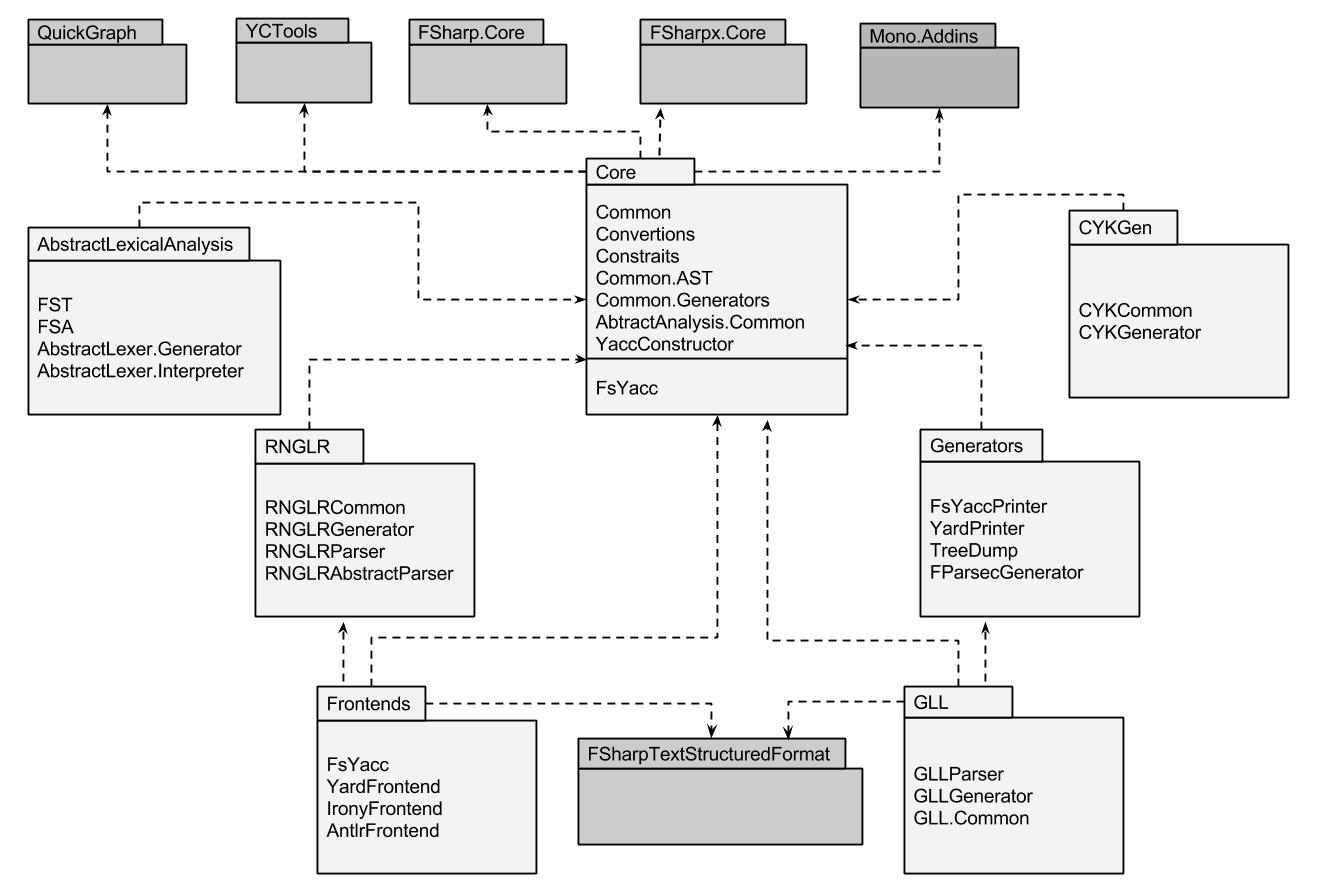
\includegraphics[scale=0.32]{Pac.jpg}}
\caption{Диаграмма пакетов. Темно серым показаны сторонние библиотеки, 
светло серым - пакеты YaccConstructor. Стрелками обозначены зависимости между пакетами.}
\end{figure}

Ниже представлено краткое описание каждого из них:
\begin{itemize}
\item Core\\
Ядро YaccConstructor: IL - внутреннее представление грамматики, преобразования грамматики и проверка корректности, управление модулями. В пакете содержится YaccConstructor.exe, с помощью которого осуществляется запуск конкретного инструмента.
\item Generators\\
Генератор (бэкенд) - инструмент, генерерующий из внутреннего представления грамматики (IL) дерево разбора, код на языке FSharp и т.д. Пакет содержит следующие генераторы: FsYaccPrinter, YardPrinter, TreeDump, FParsecGenerator. 
\item Frontends\\
Фронтенд - модуль, транслирующий представление грамматики в IL согласно языку спецификации грамматики. Пакет содержит FsYacc, YardFrontend, IronyFrontend и AntlrFrontend. 
\item RNGLR\\
Генератор, который согласно описанной грамматике создает восходящий парсер, основанный на алгоритме RNGLR. Работает с контекстно-свободными грамматиками.
\item GLL\\
Генератор, который создает нисходящий парсер для работы с неоднозначными грамматиками, а так же для разбора контекстно-свободных грамматик, включая леворекурсивные. 
\item AbstractLexicalAnalysis\\
Генератор лексических анализаторов, основанных на  конечном преобразователе (finite state transducer - FST), для разбора встроенных языков. 
\item CYK\\
Генератор, который создает восходящий парсер, основанный на алгоритме CYK. Работает с контекстно-свободными грамматиками.
\end{itemize}

Для каждого пакета на языке XML написан файл спецификации (NuSpec). В нем указан путь к исполняемым файлам и библиотекам, которые должны быть собраны в пакет, а также зависимые библиотеки или пакеты. Зависимые библиотеки - библиотеки, необходимые для работы данного пакета. При установке пакета зависимые библиотеки автоматически устанавливаются в тот же проект решения, что и данный пакет. Также в nuspec присутствует краткое описание пакета, указан автор, версия, тэги для поиска, и т.д.

Для использования какого-либо модуля требуется запуск YaccConstructor.exe. Чтобы обеспечить видимость модулей после установки пакетов в решение, были внесены изменения в файл YaccConstructor.addins, который собирается в пакет Core.  В этом файле указан путь к директории, в которой будет осуществляться поиск установленных модулей. 

При наличии файлов спецификации с помощью команд nuget pack и nuget push, исполняемых из командной строки, производится сборка и публикация пакетов. 
Перед публикацией пакетов на myget.org было произведено предварительное тестирование. Выполнена локальная сборка всех пакетов и проверено наличие в пакетах всех необходимых файлов. Также  проверено, что все модули доступны для работы. 
\subsection{Настройка автоматизированной сборки} 
В YaccConstructor была реализована сборка и публикация пакетов в системе NuGet. При каждом запуске сборки проекта на сервере TeamCity в файле с хранимой версией производится инкремент разряда версии сборки. Эта версия с приписанным к ней суффиксом -On-branch--local проставляется во все файлы спецификации. \\
Внесены изменения в скрипты сборки, для того, чтобы при сборке пакетов не происходило переименования имен исполняемых файлов в папке Bin/Release. \\
Сборка и публикация пакета YC.Tools, реализованые в проекте, были внесены в общую сборку пакетов. Файл спецификации YC.Tools помещен в единую директорию с файлами спецификации выделенных пакетов. 
\subsection{Тестирование}
Тестирование полученного решения было проведено на примере среды разработки - IDE (Integrated development environment) для параллельного вычислителя, построенного на виртуальной архитектуре. Из исходного кода на ассемблере требуется получить дерево разбора, с которым будет работать интерпретатор.\\
Для проведения тестирования были выполнены следующие шаги:
\begin{itemize}
\item Бинарные пакеты, содержащие требуемые инструменты, установлены в проект.  Для данного решения выбраны YardFrontend и RNGLR генератор. Установлены пакеты YC.Core, RNGLR и Frontends. 
\item По описанной грамматике с помощью YardFrontend получили внутреннее представление грамматики.
\item На основе полученного внутреннего представления грамматики с помощью генератора RNGLR сгенерирован парсер. 
\item Полученный парсер использовали для генерации дерева разбора кода, интерпретируемого в IDE. 
\end{itemize}

% У заключения нет номера главы
\section*{Заключение}
В ходе работы были достигнуты следующие результаты:
\begin{itemize}
\item Изучена структура проекта  YaccConstructor.
\item Изучена функциональность каждого модуля, определена структура опубликованных бинарных пакетов.
\item Произведено предварительное тестирование бинарных пакетов.
\item Реализована сборка и публикация пакетов согласно разработанной структуре.
\item Проведено тестирование полученной функциональности.\\
\end{itemize}
Код опубликован в репозитории проекта YaccConstructor: \\ https://github.com/YaccConstructor.\\
Имя пользователя, под которым работал автор: VereshchaginaE



\bibliographystyle{ugost2008ls}
\bibliography{diploma.bib}
\end{document}
